\chapter{Data Pipeline}
\label{chap:data-pipeline}
\sloppy
\section{Introduction}
This chapter provides a detailed overview of how the data was sourced, processed, and prepped for two inputs, proteins and drugs, turning them from raw data to computationally readable for the model.

\section{Data Collection and Curation}
Data is an extremely important part of this project, and it's important to gather a sufficient amount of scientifically accurate data so the model can be the most accurate as possible.
This section will define how the data was sourced and manipulated to reach its final representation.
\subsection{Primary Data Source}
I extracted the initial bulk of my data from BindingDB \citep{bindingdb_web}, which is a public database holding experimentally measured binding affinities between small molecules and proteins.
BindingDB serves as a critical resource to a diverse range of applications, including development of artificial intelligence models.
The database has grown significantly, holding information on 2.9 million binding measurements for 1.3 million compounds.
Data can be extracted through its web-services or downloaded directly.
Due to the nature of the project, the initial phase begins with a local download of two raw data files to facilitate data cleaning and binarization:
\begin{itemize}
    \item \texttt{BindingDB\_all.tsv} file containing millions of interaction records
    \item \texttt{Sequences.fasta} file containing the amino acid sequences for all protein targets in the database.
\end{itemize} 
\subsection{Data Merging and Cleaning}
The raw data from BindingDB didn't contain protein sequences, making it unsuitable for feature engineering, so the first step after downloading all raw data was to unify the interaction and protein sequence data.
Using the protein name as a common key, the \texttt{.tsv} and \texttt{.fasta} file were merged, creating a unified dataset where each row contained \textbf{Drug SMILES}, \textbf{Target Sequence}, \textbf{Binding Affinity Value}, and the \textbf{Interaction classification}.

BindingDB reports binding affinity across several measurements: Ki, Kd, IC50, and EC50.
But most rows contain only one or two of these values, as illustrated in Table~\ref{tab:raw_csv}.
Ki and Kd are preferred as they measure direct binding affinity, whereas IC50 and EC50 are functional measures that depend on assay conditions, making them less directly comparable \citep{He2017}.
To maximise data coverage, we adopted a priority-based fallback: Ki is used when available, otherwise Kd, then IC50, and finally EC50.
The selected value is converted into a log-scaled representation described in Subsection~\ref{subsec:data-binarization-&-negative-sampling}, compressing the wide range of raw nanomolar values into a more stable scale, \textit{pAffinity}, for model training.
A full justification of affinity type selection is provided in Subsection~\ref{subsec:affinity-type-justification-(ki-kd-ic50)}.

Mixing heterogeneous affinity types like this is a known limitation of this approach, as the absolute values are not directly comparable across measurement types.
But it is partially mitigated with a grey-area buffer used during binarisation, to only allow confidently strong binders and clear non-binders to receive labels.

During the merge, the data was also cleaned to remove duplicate interactions, any rows with NULL values, and where affinity $\leq$ 0.
After filtering for Homo sapiens targets only, the result was a completely unified table containing the necessary information to continue with feature engineering.


A snippet of the raw \texttt{.tsv} file is shown in Table~\ref{tab:raw_csv}.
% --- TABLE 1: Raw CSV Snippet ---
\begin{table}[H]
  \centering
  \caption{Snippet from \texttt{bindingdb\_all.tsv} (Raw)}
  \label{tab:raw_csv}
  \begin{tabular}{l l l r r r r}
    \toprule
    Drug SMILES & \textbf{Target Name} & Ki (nM) & Kd (nM) & IC50 (nM) & EC50 (nM) \\
    \midrule
    \texttt{CC(=O)Oc1\ldots} & Thymidine kinase & 50.0 & --- & --- & --- \\
    \texttt{C[N]1C=C\ldots} & Thymidine kinase & --- & --- & 12000.0 & --- \\
    \texttt{CC(C)(C)OC\ldots} & ABL1 kinase & --- & 75.0 & --- & --- \\
    \bottomrule
  \end{tabular}
\end{table}
% ---------------------------------
The \texttt{.fasta} file was parsed into a key-value dictionary to map protein names to their sequences, as shown in Table~\ref{tab:fasta_parsed}.
% --- TABLE 2: Parsed FASTA Snippet ---
\begin{table}[H]
  \centering
  \caption{Example of Parsed \texttt{binddbtargetsequence.fasta} Data}
  \label{tab:fasta_parsed}
  \begin{tabular}{l l}
    \toprule
    Key (from FASTA Header) & Value (Sequence) \\
    \midrule
    \textbf{Thymidine kinase} & \texttt{MPK...} (sequence truncated) \\
    \textbf{ABL1 kinase}      & \texttt{GKL...} (sequence truncated) \\
    ...                       & ... \\
    \bottomrule
  \end{tabular}
\end{table}
% -------------------------------------
These two sources were merged on the target name.
After merging, cleaning, and binarization, the final unified dataset was created and a snippet shown in Table~\ref{tab:merged_data}.
% --- TABLE 3: Final Merged Data Snippet ---
\begin{table}[H]
  \centering
  \caption{Snippet of Final Merged and Processed Dataset}
  \label{tab:merged_data}
  \begin{tabular}{lllrl}
    \toprule
    \texttt{drug\_smiles} & \texttt{target\_sequence} & \texttt{target\_name} & \texttt{p\_affinity} & \texttt{interaction} \\
    \midrule
    \texttt{CC(=O)Oc1...} & \texttt{MPK...} & Thymidine kinase & 7.30 & 1 \\
    \texttt{C[N]1C=C...} & \texttt{MPK...} & Thymidine kinase & 4.92 & 0 \\
    \texttt{CC(C)(C)OC...} & \texttt{GKL...} & ABL1 kinase & 7.12 & 1 \\
    \bottomrule
  \end{tabular}
\end{table}
% ------------------------------------------

\subsection{Drug Identifier Normalization}
Drug identifiers provided by BindingDB corresponded to experimental compounds instead of approved and recognised drug names.
This made it difficult to use the front end as the identifiers were very lengthy and chemically descriptive.
To address this, the identifiers were normalised to be in simpler forms while being retained to ensure traceability back to the original BindingDB database.
\begin{lstlisting}[caption={drug name normalisation from BindingDB identifiers}]
def normalize_drug_name(self, name: str):
    if name is None or pd.isna(name):
        return None
    name = str(name).strip()
    if not name:
        return None
    parts = [p.strip() for p in name.split("::") if p.strip()]
    if not parts:
        return None
    parts = sorted(parts, key=len)
    for p in parts:
        if not re.search(r"[=#\[\]\(\)]", p):
            return p
    return parts[0]
\end{lstlisting}


\subsection{Affinity Type Justification (Ki, Kd, IC50)}
\label{subsec:affinity-type-justification-(ki-kd-ic50)}
BindingDB already provides some experimentally measured binding affinity types, such as \textit{Ki}, \textit{Kd}, and \textit{IC50}.
Although these quantities are related, they do not supply us with meaning and are not suitable to begin our classification of the dataset.
\subsubsection{Definitions and Mechanistic Differences}
\textbf{Ki} (inhibition) measures the binding between an inhibitor drug to an enzyme, which strictly reduces the catalytic activity of the enzyme.
\textbf{Kd} (dissociation) also measures the binding equilibrium between a drug and protein but in a more general, all-encompassing term to include all the dissociated components.
Both Ki and Kd are equilibrium constants governed by the same thermodynamic principles \citep{sciencesnail_ki_kd}.
\textbf{IC50} is short for inhibitory concentration 50\%, meaning the concentration of inhibitor required to reduce the biological activity of interest to half of the uninhibited value.
The simplicity and lack of assumptions required to generate these data make them useful, but as it doesn't directly measure the binding equilibrium, it is a less accurate measurement than Ki or Kd. The relationship between IC50 and Ki is described by the Cheng-Prusoff equation, which shows that IC50 varies with substrate concentration even when Ki remains constant \citep{cheng_prusoff}.
\textbf{EC50} stands for effective concentration 50\%, which refers to the concentration of drug at which 50\% of its maximum effect is achieved.
Making it more effective for experiments wanting the dosage to be quantified even when the enzyme activity doesn't reach the 50\% threshold causing IC50 to be undefined.
It reflects functional activity rather than direct binding affinity.
EC50 measurements incorporate complex factors including receptor reserve, signal transduction efficiency, and cellular response mechanisms \citep{sciencesnail_ki_kd}.
\subsubsection{Justification for Ki Selection}
To evaluate which affinity type is most appropriate for my model, we analysed the BindingDB dataset across four key criteria: mechanistic validity, data quality, measurement reliability, and data availability.
\textbf{Mechanistic Validity:} Ki and Kd represent true equilibrium binding constants that are substrate-independent and thermodynamically well-defined.
In contrast, IC50 and EC50 are functional assays whose values depend on experimental conditions and do not directly measure binding affinity.
For a machine learning model intended to learn binding relationships, using equilibrium constants provides a more robust and interpretable basis (Figure~\ref{fig:ki_justification}A).
\textbf{Data Quality:} After reviewing the graphs generated from the raw bindingDB file, Ki has the lowest outlier rate, which indicates more consistent experimental measurements compared to IC50 and Kd. Higher consistency is better for training the model as it's reducing noisy and inconsistent labels from the dataset (Figure~\ref{fig:ki_justification}B).
\textbf{Data Availability:} While IC50 measurements are more abundant in BindingDB (47,043 entries), Ki still provides 16,796 high-quality measurements.
This is plenty to develop and train machine learning models as modern deep learning models have shown it's more valuable to have high-quality data than a higher quantity \citep{data_quality_ml}.
\textbf{Cross-Validation with Correlation Analysis:} To confirm the relationships between affinity types, a correlation heatmap was generated across all measurements in the raw BindingDB dataset (Figure~\ref{fig:corr_heatmap}). The high correlation between Ki and Kd (r = 0.94) confirms their mechanistic similarity as equilibrium constants.
The moderate correlation between Ki and IC50 (r = 0.81) reflects IC50's dependence on experimental conditions, while the weaker correlation with EC50 (r = 0.55) highlights its distinct mechanistic basis as a measure of functional activity rather than binding affinity.
\begin{figure}[H]
    \centering
    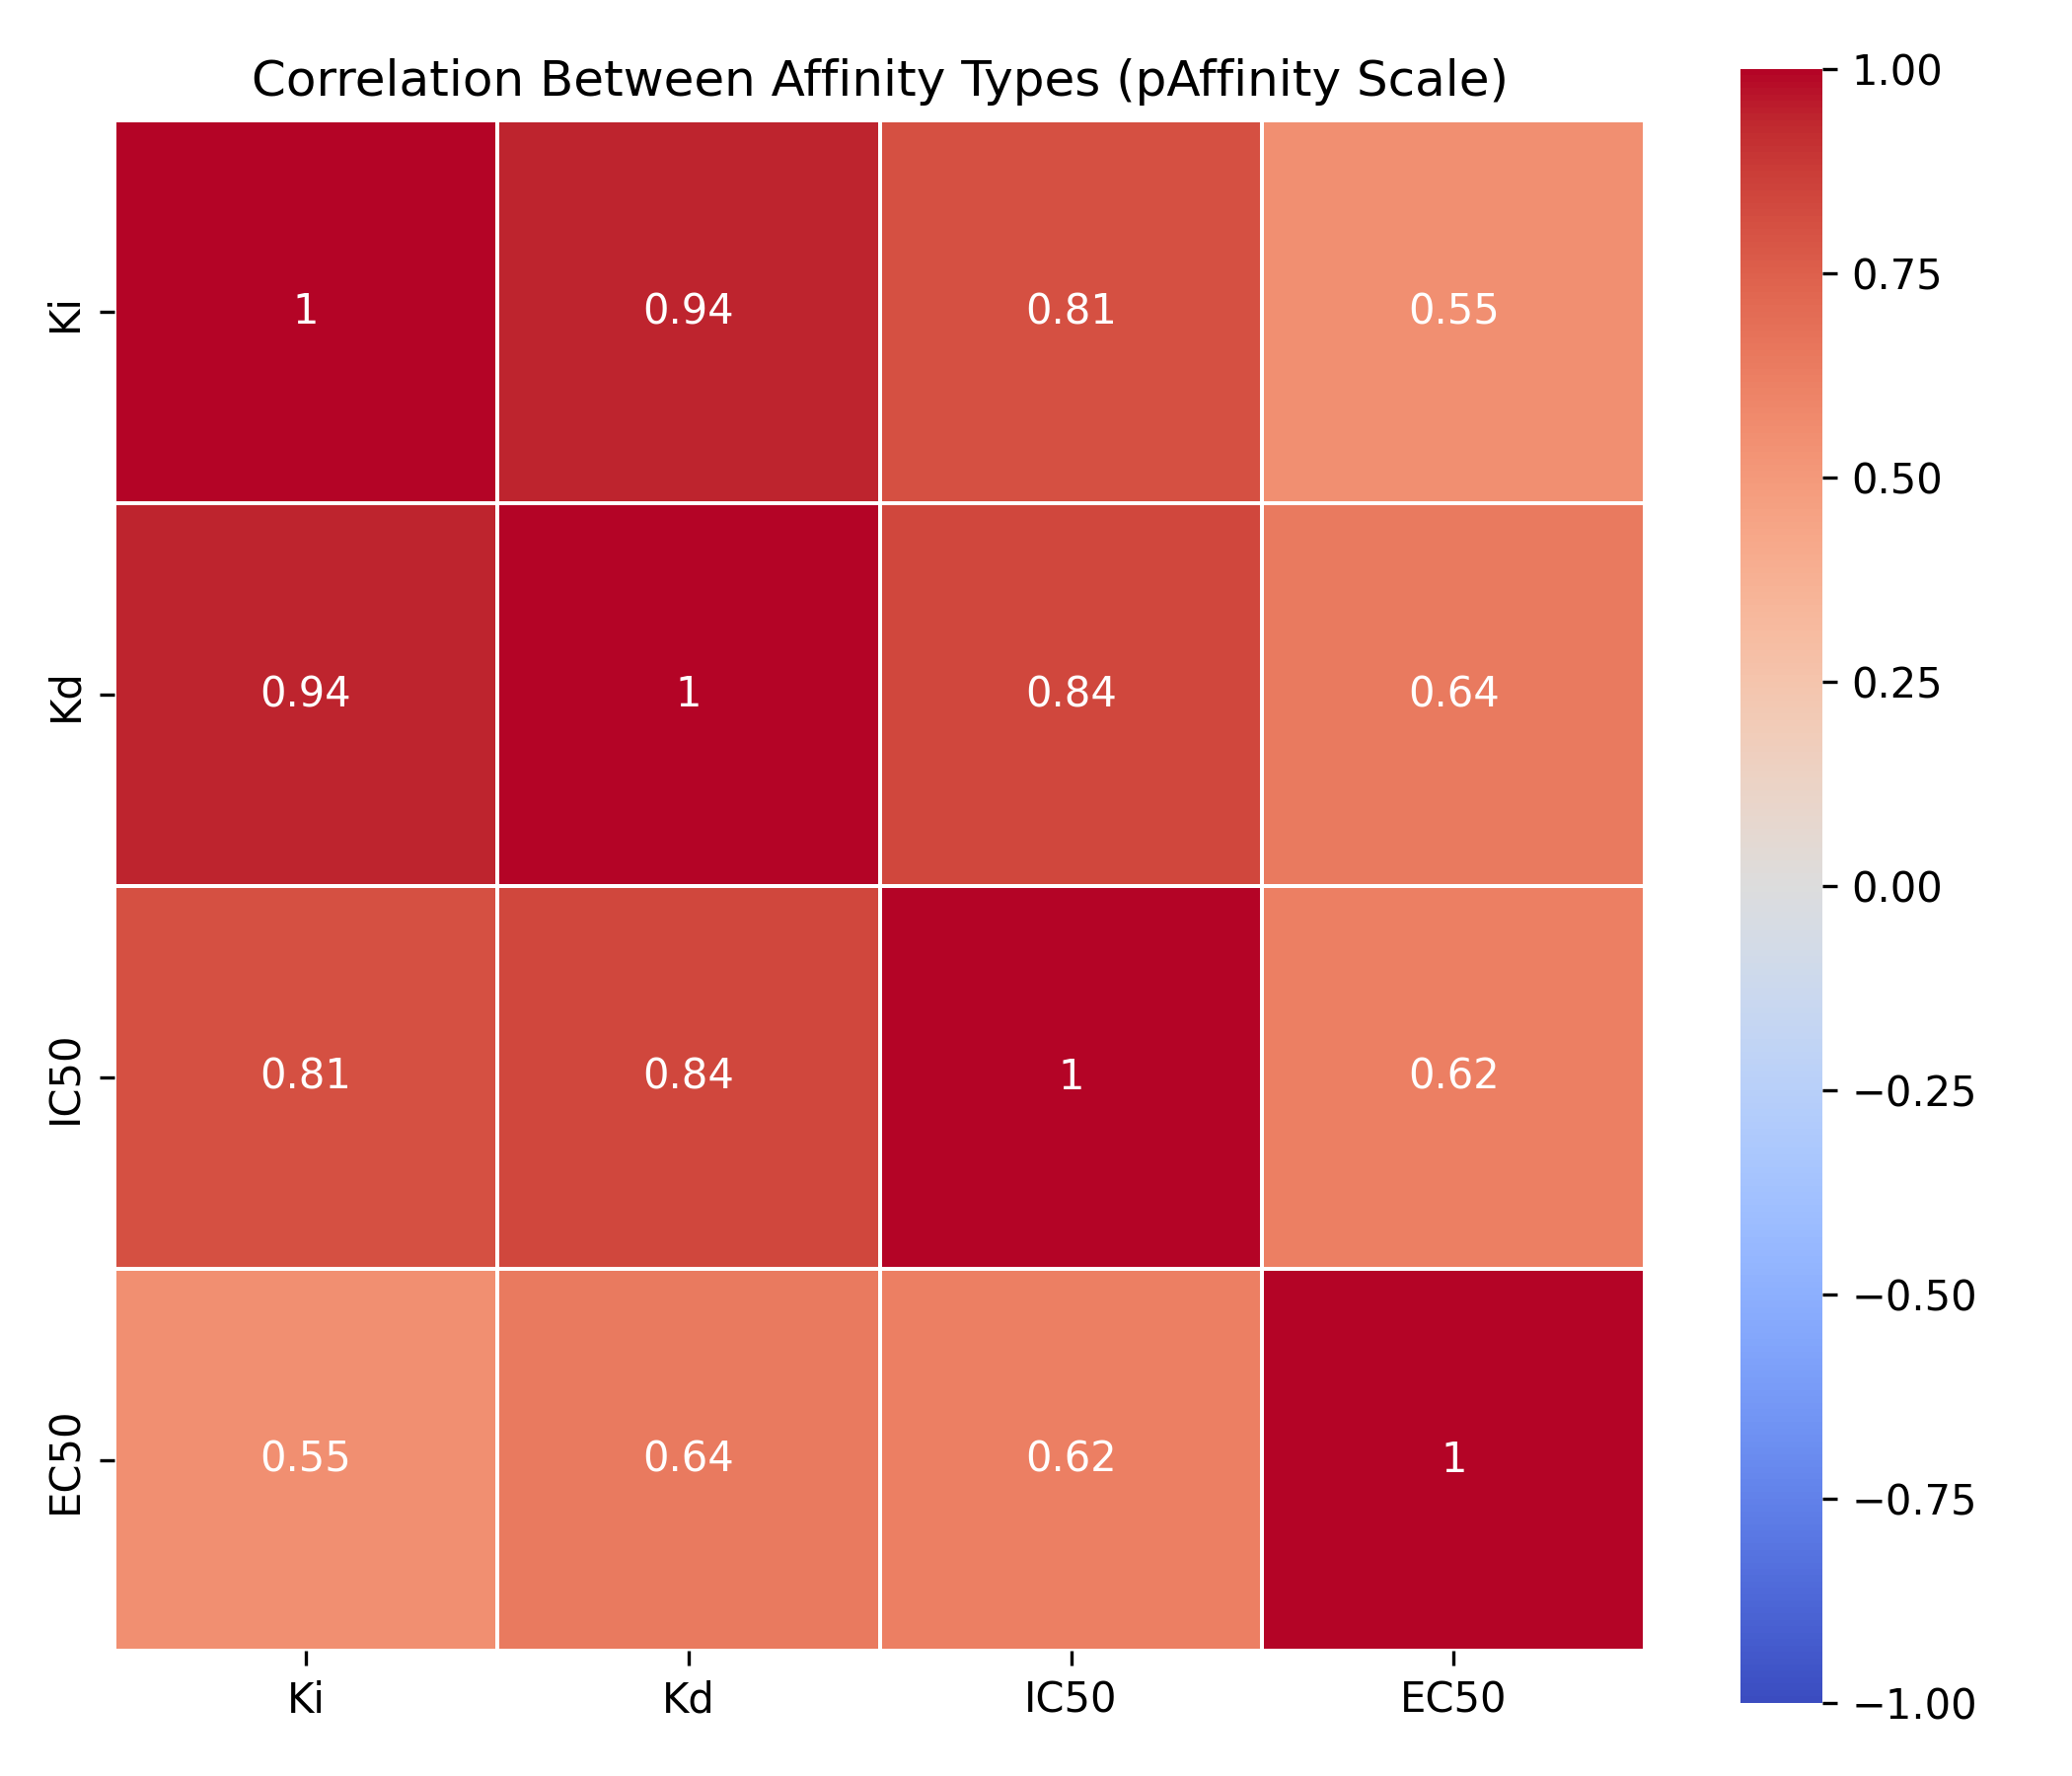
\includegraphics[width=\textwidth]{affinity_correlation_heatmap.png}
    \caption{Heatmap showing the correlation between the different affinity values to show similarities in the values given}
    \label{fig:corr_heatmap}
\end{figure}
Based on this analysis, \textbf{Ki was selected as the primary affinity measurement} followed by Kd then IC50 as Kd will provide more accurate data than IC50, but it is not present enough to be used initially.
Ki provides the perfect balance of mechanistic validity (true equilibrium constant), data quality (lowest measurement variability), and sufficient quantity (16,796 measurements) for reliable DTI classification.
\begin{figure}[H]
    \centering
    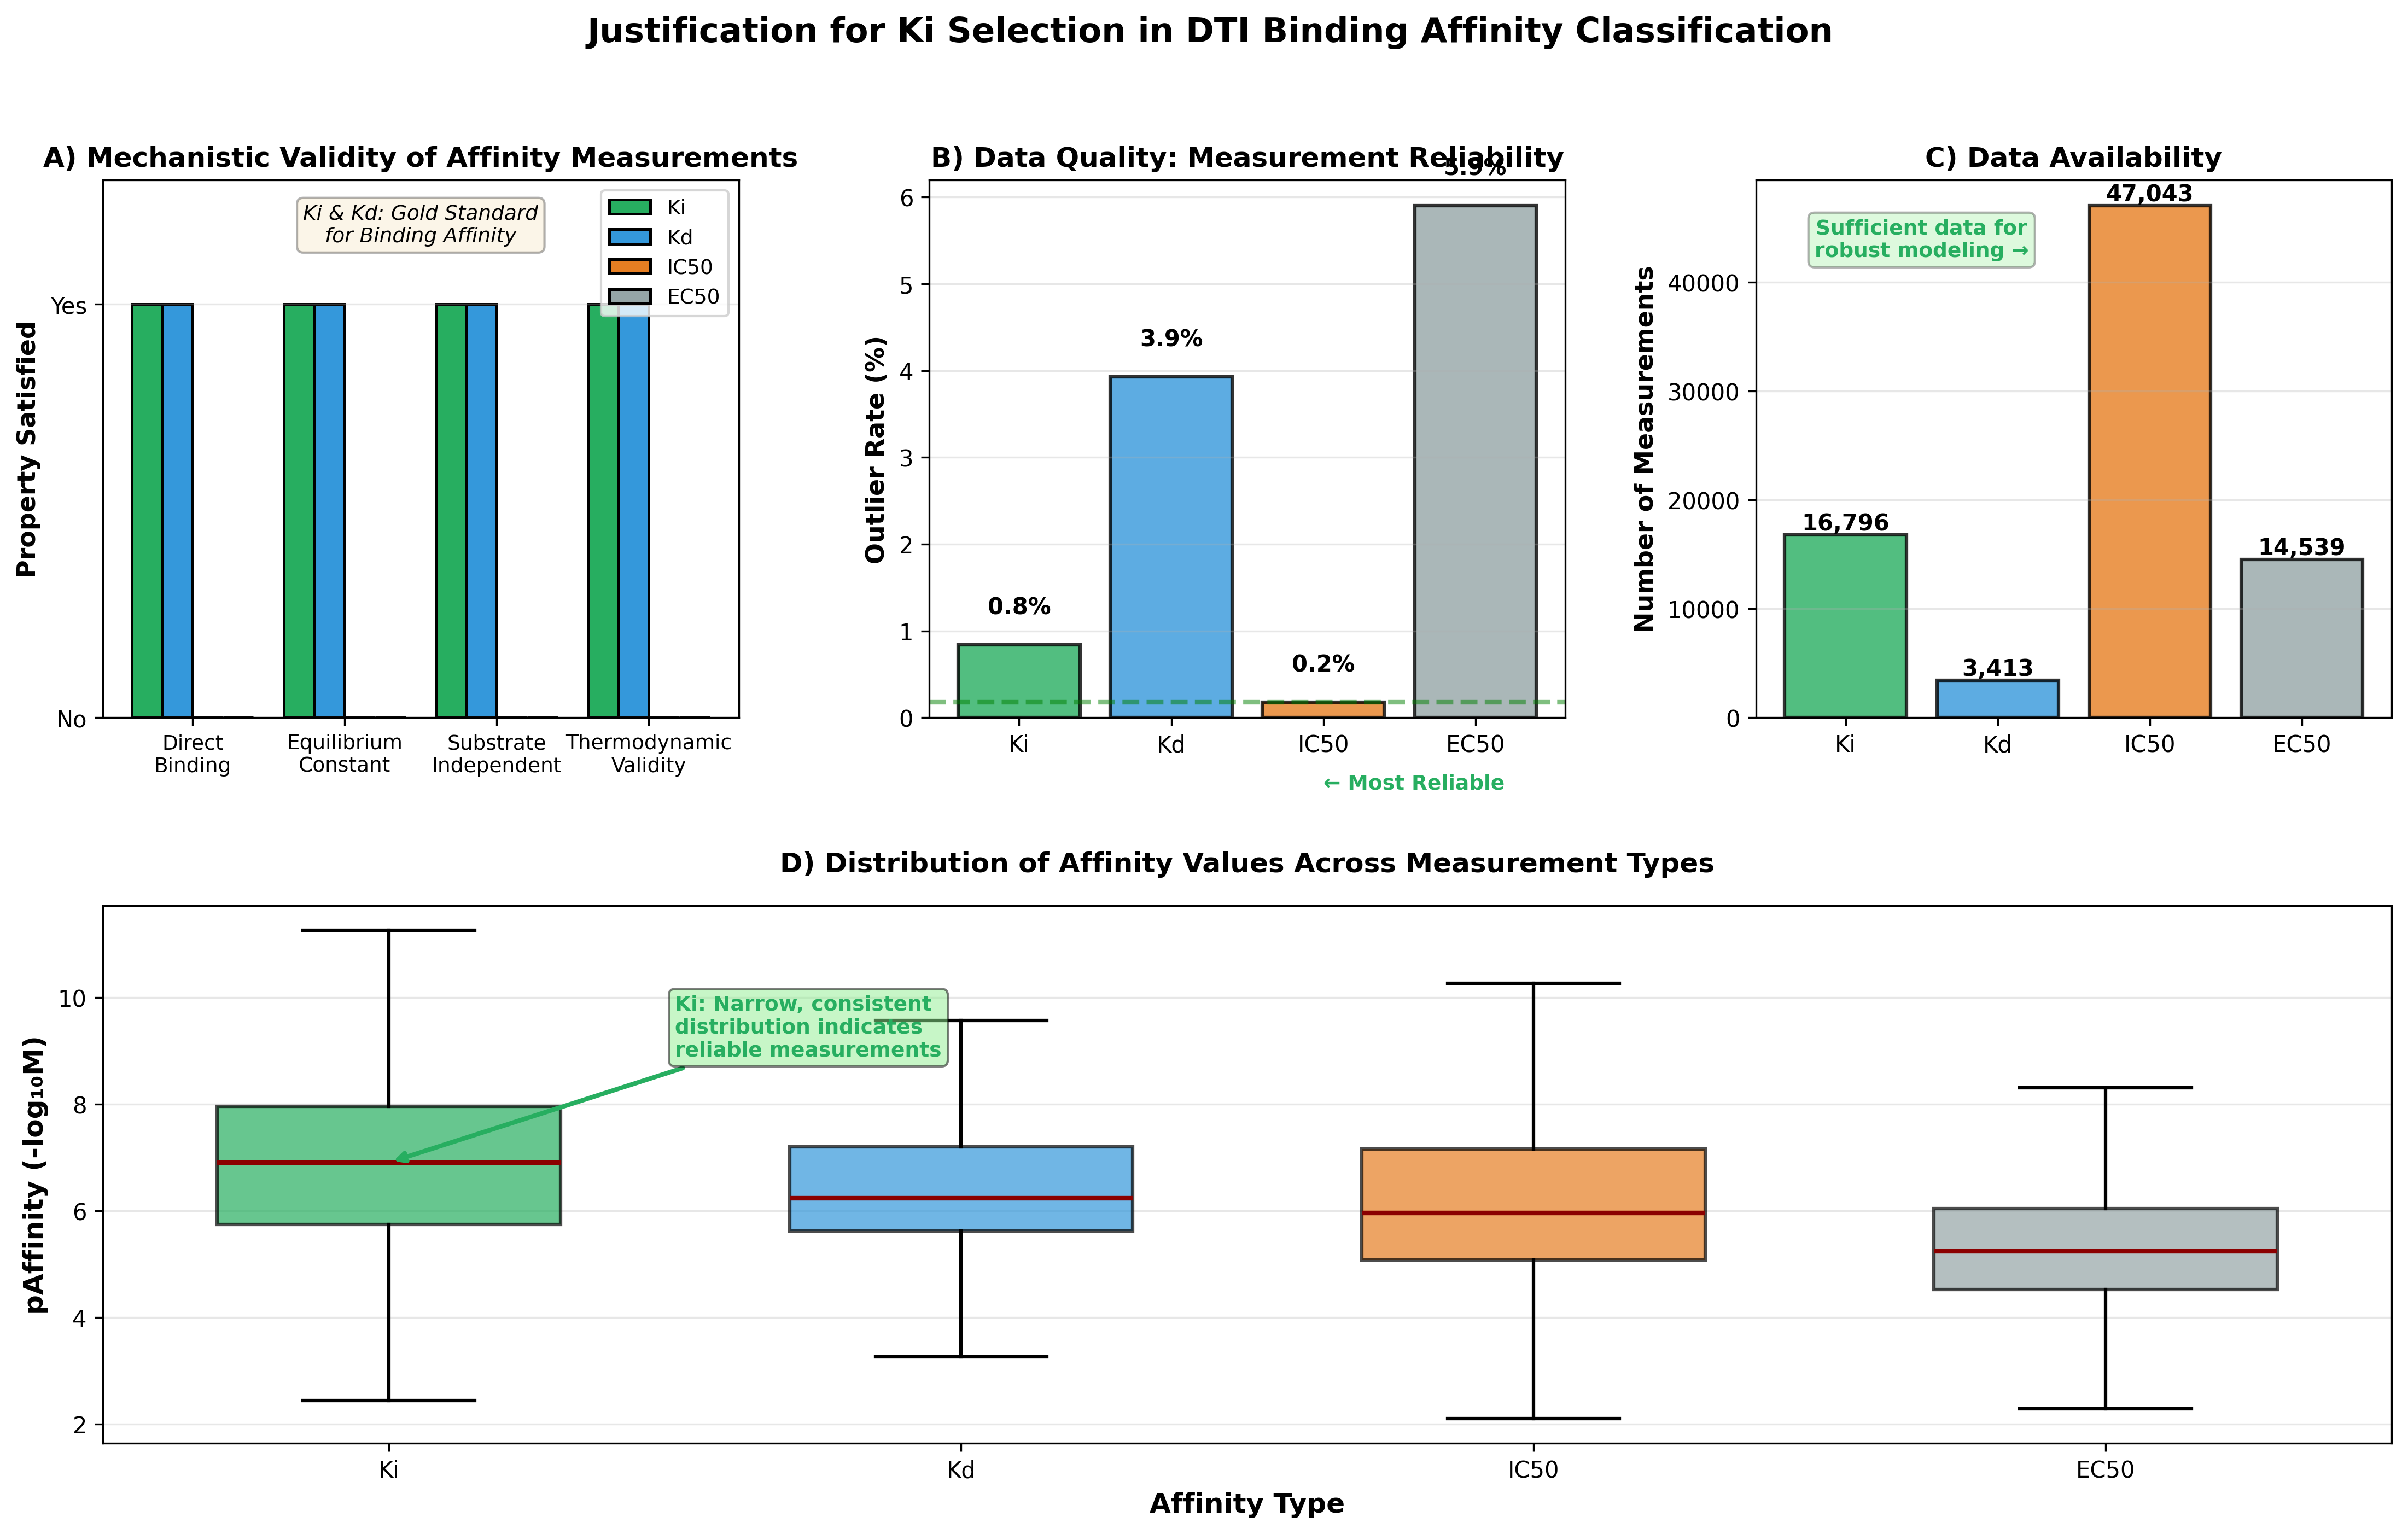
\includegraphics[width=\textwidth]{ki_justification_comprehensive.png}
    \caption{Comprehensive justification for Ki selection. (A) Mechanistic validity comparison showing Ki and Kd satisfy all criteria for true binding measurements. (B) Data quality assessment via outlier rates. (C) Data availability across affinity types. (D) Distribution of pAffinity values showing Ki's consistent measurement characteristics.}
    \label{fig:ki_justification}
\end{figure}

\subsection{Data Binarization \& Negative Sampling}
\label{subsec:data-binarization-&-negative-sampling}
It's crucial to classify the data accurately with meaningful representations and thresholds.
From the BindingDB dataset we used the columns \textbf{Ki} \& \textit{Kd} and set thresholds on this value to determine the score binder or non-binder.
Instead of using raw nanomolar (nm) values, the binding affinities were transformed into their log-scaled form using equation~\ref{eq:paffinity}:
\begin{equation}
\mathrm{pAffinity} = -\log_{10}\left( \mathrm{Affinity\,(M)} \right)
\label{eq:paffinity}
\end{equation}

Where the raw nanomolar (nM) value is first converted to molar (M) units using equation~\ref{eq:nm_to_m}:

\begin{equation}
\mathrm{Affinity\,(M)} = \mathrm{Affinity\,(nM)} \times 10^{-9}
\label{eq:nm_to_m}
\end{equation}
This representation is widely used in the industry and literature \citep{Thafar2022, DSouza2023, He2017, Ozturk2018} due to its biological interpretability and numerical stability.

A common challenge with data in DTI is the insufficient number of true negative data as databases are biased towards successful binding experiments.
A basic solution to this is random negative sampling, which pairs drugs and proteins at random and assuming they do not interact.
However, this can introduce a high rate of false negatives and degrade model performance, which is highlighted as an issue of \textit{low-confidence negative samples} in \citep{bai2021hierarchical}.
Methods like fuzzy-rough approximation \citep{islam2021dti}, select negatives by degree rather than at random, providing a better alternative for this type of sampling.

To counter this issue, we defined two binding thresholds and used negative sampling with care by following the \textit{safe-margin} practice described in \citep{bai2021hierarchical}.
Therefore, we classify pairs with pAffinity value $>$ 7 as a binding interaction (label = 1), and pairs with pAffinity value $<$ 5.3 as non-binding (label = 0).

\subsection{Implementation of Affinity Transformation and Label Assignment}
\begin{lstlisting}[caption={Affinity transformation and binary label assignment}]
    df_chunk = df_chunk[df_chunk['affinity_value_nm'] > 0].copy()
    # Convert to pAffinity (-log10)
    df_chunk['p_affinity'] = -np.log10(df_chunk['affinity_value_nm'] * 1e-9)
    # Create Binary Labels (-1 = invalid, 0 = non-binder, 1 = binder)
    df_chunk['interaction'] = -1
    df_chunk.loc[df_chunk['p_affinity'] > BINDER_THRESHOLD_P, 'interaction'] = 1
    df_chunk.loc[df_chunk['p_affinity'] < NONBINDER_THRESHOLD_P, 'interaction'] = 0
    # Keep only valid 0 or 1
    df_chunk = df_chunk[df_chunk['interaction'].isin([0, 1])]
\end{lstlisting}

This approach generates an area between the thresholds, which represents an ambiguous \textit{grey area}, a zone where the interactions are too week to be a binder but too strong to be a clear non-binder.
To increase the performance of the model, we only want to train it on the clearest signals, so all pairs inside the \textit{grey area} are removed from the loaded dataset shown in Table~\ref{tab:dataset-before-threshold}, and a distribution graph visualising the grey area is shown below in Figure~\ref{fig:affinity_dist}.

\begin{figure}[H]
    \centering
    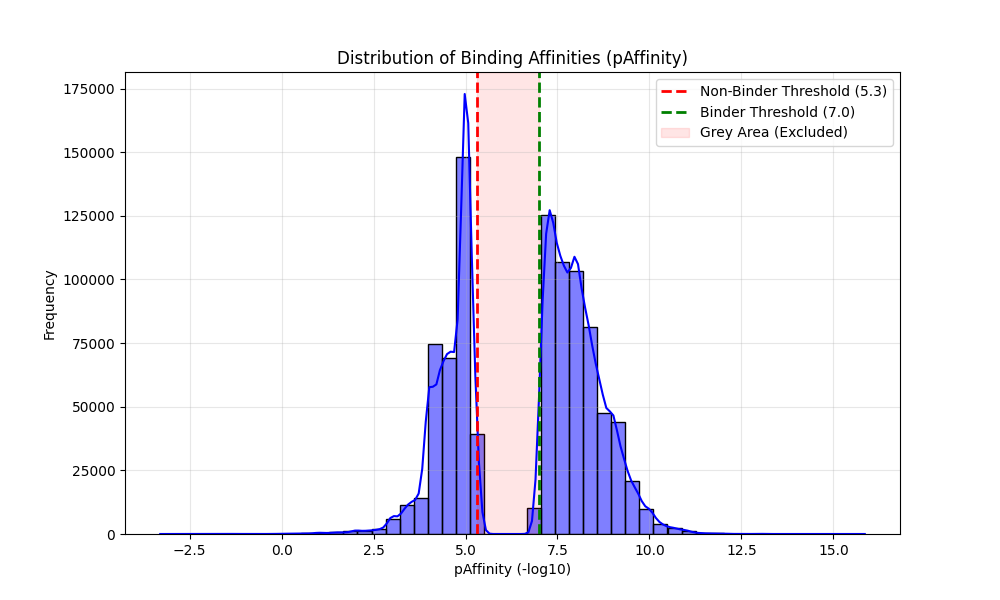
\includegraphics[width=0.8\textwidth]{affinity_distribution.png}
    \caption{Distribution of pAffinity values in the filtered dataset. The red shaded region represents the \textit{Grey Area} ($5.3 \le \mathrm{pAffinity} \le 7.0$), where data points were excluded to ensure high-confidence labels.}
    \label{fig:affinity_dist}
\end{figure}

\begin{table}[htbp]
\centering
\caption{BindingDB Dataset Summary Before Thresholding}
\label{tab:dataset-before-threshold}
\begin{tabular}{lrc}
\toprule
\textbf{Metric} & \textbf{Count} & \textbf{Percentage} \\
\midrule
Total interaction pairs                          & 1,416,025 & --      \\
Binders (pAffinity $> 7.0$)                      & 552,618   & 39.03\% \\
Non-binders (pAffinity $< 5.3$)                  & 356,025   & 25.14\% \\
Grey area ($5.3 \leq$pAffinity $\leq 7.0$)      & 507,382   & 35.83\% \\
\bottomrule
\end{tabular}
\end{table}

After removing the 507,382 pairs falling within the grey area, the remaining interactions were assigned binary labels, resulting in the class distribution shown in the Table~\ref{tab:class-distribution1}.
\begin{table}[H]
\centering
\caption{Final Class Distribution After Thresholding}
\label{tab:class-distribution1}
\begin{tabular}{cllrc}
\toprule
\textbf{Class Label} & \textbf{Interaction Type} & \textbf{Threshold Criteria} & \textbf{Count} & \textbf{Percentage} \\
\midrule
1     & Binder (Positive)      & pAffinity $> 7.0$ & 552,618 & 60.82\% \\
0     & Non-Binder (Negative)  & pAffinity $< 5.3$ & 356,025 & 39.18\% \\
\midrule
\textbf{Total} & & & \textbf{908,643} & \textbf{100\%} \\
\bottomrule
\end{tabular}
\end{table}
A subsampled copy with 18.5k interactions was used for the iterative experiments to be compatible with NumPy backpropogation.
This was split train/val/text as 12,038/3,704/2,778, and the distribution was mentioned in Table~\ref{tab:class-distribution} in the evaluation section.

\section{Feature Engineering}
This section outlines the Feature engineering process to turn raw chemical and biological data into machine-readable formats.
Drug SMILES and Target Sequences must be encoded into fixed-size numerical vectors as neural networks cannot process the raw text representations.
\subsection{Drug Representation}
Drug SMILES being represented as variable length strings are unsuitable for the model to ingest.
To address this issue, drug SMILES were encoded into MACCS keys, a 167-bit binary fingerprint, where each bit represents the presence of a different chemical substructure.
\subsection{RDKit}
The open-source Cheminformatics toolkit RDKit performed \textit{Descriptor Generation} by parsing SMILES strings into \textit{Mol objects}, translating complex chemical structures into a fixed length vector (MACCS Keys) that the model can use to learn patterns for each drug \& protein pair \citep{rdkit_doc}.
As a vector notation:
\[
\text{MACCS} = [0,0,1,0,0,0,0,0,\,1,0,0,0,0,0,0,0,\,1,0,1,\dots] \in \{0,1\}^{167}.
\]
\subsection{Protein Representation} 
The Proteins are represented as amino acid sequences of varying lengths, often exceeding thousands of characters.
To normalise the sequences, so they're suitable for the neural network, the variable-length sequences were converted into fixed-size continuous embeddings.
\subsection{ProtBERT}
To ensure the embeddings were as accurate as possible, ProtBERT was used as it's a pretrained transformer model based off of the BERT architecture \citep{devlin2019bertpretrainingdeepbidirectional}.
ProtBERT understands the contextual and biophysical properties of the amino-acid sequences as it has been trained on a huge database of protein sequences UniRef100 \citep{UniProt2025} containing 217 million sequences \citep{Elnaggar2020.07.12.199554}.
By extracting the hidden states from the model through mean pooling, each protein sequence is condensed into a semantic vector embedding that fits the fixed-size, \textit{1024 floating-point values}, input and preserves the biological context, such as 3D structure or chemical polarity \citep{ProtBERT}.

Protein embedding (example, size 1024):
\[
\mathbf{p}_{\text{ex}} \in \mathbb{R}^{1024} =
[\,0.320856,\,-0.685886,\,-0.652373,\ldots,\,-0.344068]
\]

\section{Data Preparation}
Following feature engineering, the processed data was split into 3: \textit{Training, Validation} and \textit{Testing}.
This is an important step to prevent overfitting of the model on the dataset, keeping this randomised is key to the validity of the model.
\subsection{Train-Validation-Test Split Methodology}
To ensure reproducibility, the dataset was split similarly to \citep{Nunes2019, Lorenz2019}at a ratio of 65:20:15.
To make it a random sampling approach, a fixed random seed (random\_state = 42) was used to make the sampling procedure deterministic, meaning each run produces the same split.
This is important for reliable model evaluation, comparison between experiments, and debugging.
The splitting was split into two stages:
\begin{itemize}
    \item \textbf{Primary Split} – The merged dataset was split into a 65\% for Training and 35\% for a Secondary set.
    \item \textbf{Secondary Split} – The secondary set of data was split to 57.14\% and 42.86\% to get the overall split of 20\% for validation and 15\% for testing.
\end{itemize}

\begin{table}[htbp]
\centering
\caption{Dataset Partitioning (65:20:15 Split)}
\label{tab:dataset-split}
\begin{tabular}{lcr}
\toprule
\textbf{Subset} & \textbf{Split \%} & \textbf{Sample Count} \\
\midrule
Training   & 65\% & 590,617 \\
Validation & 20\% & 181,729 \\
Testing    & 15\% & 136,297 \\
\bottomrule
\end{tabular}
\end{table}
\subsection{Justification of Split Ratios}
While an 80:20 ratio between training and testing is common \citep{Talukder2025, Zhan2025}, A higher validation set of data at 20\% was used for more accurate estimates of model performance during training.
This can allow for better hyperparameter tuning so the model can be tweaked to optimise performance on the unseen test data.
This specific split has been used among other deep learning studies that require rigorous hyperparameter tuning, such as in medical image analysis \citep{Nunes2019} and environmental prediction modelling \citep{Lorenz2019}.
A large allowance to the validation set reduces the risk of overfitting before the final evaluation on the unseen test data.








